\documentclass{article} 

\usepackage[french]{babel}
\usepackage[utf8]{inputenc}
\usepackage[T1]{fontenc}
\usepackage{amsmath}
\usepackage{graphicx}
\usepackage{float}
\usepackage[right=2.5cm,left=2.5cm,bottom=2.5cm,top=2.5cm]{geometry}
\title{Tutos: comment programmer une fusée}
\author{Alexis Vandewalle}
\usepackage{program}

\begin{document}
\maketitle
\section{Clonage des fichiers du Scube}
Les codes utilisé pour pour la fusée sont stocké sur un serveur de l'école. Nous utilisons un logiciel de
gestion de version nommé git afin de gérer les versions des codes et de mettre sur le serveur les fichiers.
Il y a deux répertoires git qui sont situés aux adresses suivantes:
\begin{itemize}
\item \verb"https://openforge.isae.fr/git/sources_raspi" (codes pour la raspberry)
\item \verb"https://openforge.isae.fr/git/sources_pic" (codes pour les micro-contrôleurs)
\end{itemize}
Pour copier ces répertoires utiliser entrer la commande \verb"git clone adresse".

\section{Programmation d'un microcontoleur de type dspic33ep256mc502}
\subsection{Matériel nécessaire}
Ce sont les microcontroleurs qui sont utilisé pour contrôler la plupart des fonctions de la fusée.
Pour débuter dans la programmation de ceux-ci, il faut vous munir d'une carte de prototypage comme celle-ci.
Ensuite, vous devez installer le logiciel Mplab sur votre pc.

\begin{figure}[H]
    \centering
    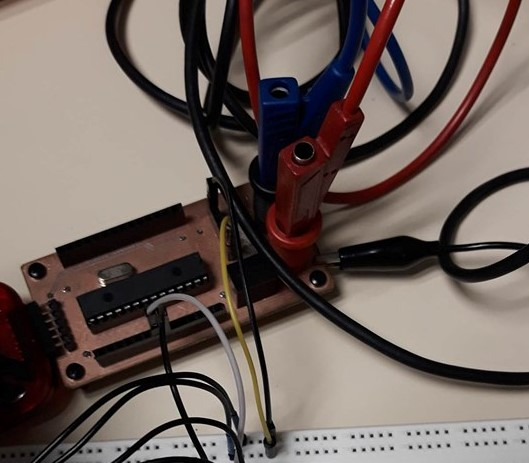
\includegraphics[width=7cm]{carteProto}
	\caption{carte de prototypage}
	\label{carteProto}
\end{figure}

\subsection{Utilisation du logiciel Mplab}
Mplab est le logiciel qui vous permettra de coder en c votre application puis de transférer celle-ci
sur votre microcontroleur.

Pour créer une application, vous devez créer un projet sur Mplab puis le configurer. Pour cela,
suivez les étapes suivantes:
\begin{enumerate}
\item file -> new project -> standalone project -> dspic33ep256mc502 -> next -> selectionner l'unique compilateur possible->finish.
\item ajouter ensuite le fichier $config\_bits.c$ (faire un copier coller de celui d'un projet existant) dans le repertoire projet, puis ajouter le dans le mplab.
\item configurer ensuite la frequence du microcontroleur: clic droit sur le projet->properties-> XC16-> define common macros->ajouter la ligne $CPU\_FREQ=16000000$ (sauf si on utilise un moteur, dans ce cas c'est $128000000$ et voir $herkulex\_controller.h$ pour plus de détails)
\item coder ensuite votre code en mettant. Pour ajoute une librairie, copier le .c et le .h dans
le répertoire du projet et ajouter les ensuite dans mplab.
\item pour téléverser votre code, cliquer sur le bouton avec un carré bleu et une flèche verte vers le bas.
\end{enumerate}

\subsection{Suivi du déroulement d'un programme}
Une des manières d'observer le bon déroulement d'un programme est d'utiliser l'interface uart sur la photo ci-dessous.
Pour l'utiliser, il suffit de brancher les TX et RX en croisé d'un point de vue physique. 
Du point de vue du code, il faut utiliser la bibliothèque serial pour le pic dans laquelle est décrite la 
procédure à suivre pour envoyer des messages.

\section{Programmation des microcontroleurs sur la case electronique}
Pour programmer un des microcontroleurs, il suffit de retirer la carte sur laquelle est placée
le microcontroleur à programmer. Ensuite, il faut le carte dont l'image est ci-dessous, la brancher
à la carte à programmer. Ensuite, on met l'alimentation puis on programme comme avec les autres microcontroleurs.

\begin{figure}[H]
    \centering
    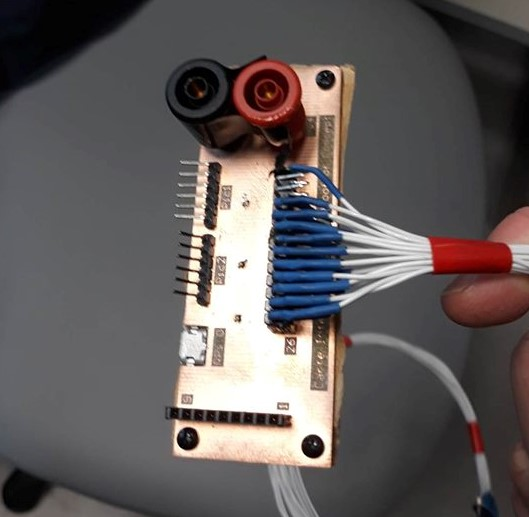
\includegraphics[width=7cm]{transfertCarteExpe}
	\caption{carte de transfert des programmes sur une carte de la case elec.}
	\label{carteTransfertExpe}
\end{figure}

\section{Programmation d'une Raspberry}
\subsection*{Installation de l'os et configuration}
Pour installer l'os sur la raspberry, suivez les étapes suivantes:
\begin{enumerate}
\item Sur votre pc installer SD card Formater et Win32DiskImager 
\item Ensuite formater la carte avec SD Card Formater 
\item Avec Win32DiskImager copier l'image iso situe dans raspberry os/raspbian\_lite\_latest
\item Copier ensuite les fichier de configuration sur la carte sd
\item Enfin, allumer votre partage de connexion et modifier le fichier de configuration wpa\_supplicant.conf en entrant vos paramètres de réseaux dans ssid(le nom du réseau) et dans psk (la clé de sécurité). Attention,
ces deux champs doivent être entre guillemet.
\end{enumerate}

Vous pouvez alors allumer la raspberry qui doit se connecter à votre réseau.

\subsection*{Se connecter a la raspberry avec le protocole ssh}
Le protocole ssh permet d'ouvrir une commande sur votre ordinateur et d'entrer des commandes qui seront
exécutées sur la raspberry depuis celui-ci. Pour se faire, il suffit de suivre les étapes suivantes:
\begin{enumerate}
\item installer le logiciel putty et le lancer
\item récupérer l'adresse ip de la raspberry dans les paramètres de partage de connexion
\item copier cette adresse dans putty
\item cocher ssh et sélectionner le port 22 et lancer le ssh
\item entrer le nom d'utilisateur(par défaut "pi") et entrer le mot de passe(par défaut "raspberry")
\end{enumerate}

\subsection*{Utiliser le bus can et programmer en c}
Voir le tuto de Damien dans sources\_raspi. Un conseil, tout de même il faut souvent précéder les
commandes de sudo lorsque le message "permission denied" apparait. Une fois cela fait, vous pouvez essayer
d'exécuter le code blink situé dans un exemple de la documentation de la bibliothèque sources\_raspi.
 
\section{les programmes déjà codé en bref}
\subsection{le programme exécuté par la raspberry de la carte expérience}
La raspberry a trois fonctions principales:
\begin{enumerate}
\item elle collecte les données des microcontrolleurs et les enregistre
\item elle détecte l'arrachage de l'ombilical
\item elle envoie certaine données à la station sol.
\end{enumerate}

\textbf{voici les actions qu'il exécute en langage naturelle:}
\begin{verbatim}
déclaration des variables utilisées
initialisation de la bibliothèque pour la gestion des pins
  si l'omilical est présent
    etat = au sol
  sinon
    etat = configuration au sol
initialisation du can et des fichiers de sauvegarde
boucle infinie
  si la télémétrie n'est pas initialisée
    on l'initialise
    on dit la configure comme transmetteur
    si etat == au sol
      on règle le temps du prochain check de la télémétrie a un certain temps
    sinon si etat == configuration au sol
      on règle le temps du prochain check de la télémétrie a un autre temps
  si etat == ground
    si l'ombilical est présent
      date de décollage = le temps actuel
      etat = en vol
  si etat == en vol
    si la duree du vol > delai d'extinction
      on éteint la télémétrie et on ferme le gestionnaire de pins
  
  si on a recu une trame sur le bus can
    on écrit la donnée dans un fichier can_file
    on switch sur l'id de la donnée
      cas TRAJ_LOG_CAN_ID
        on écrit la donnée dans un fichier log
        on l'écrit dans la file d'attente de la télémétrie
      cas SEQ_RECU_BARO_CAN_ID
        on écrit la pression dans le fichier de pression
      cas SEQ_CHUT_BARO_CAN_ID
        on écrit la pression dans un autre fichier de pression
      cas header de trajectoire
        on stocke le type de la donnée dans une variable
      cas TRAJ_DATA_CAN_ID
        selon le type de header
          on écrit la donnée dans le bon fichier
          on écrit la donnée dans la file d'attente de la télémétrie
  si la télémétrie est initialisée et que le temps>temps du prochain check
    on règle le temps du prochain check
    si le transmetteur est disponible
      si il y a des logs dans la file d'attente des logs a transmettre, on les envoie
      sinon
        on transmet le contenu de la file d'attente de donnée
\end{verbatim}

\subsection*{Le séquenceur d'éjection}
\begin{verbatim}
initialisation du pic et des capteurs du pic
boucle infinie:
  lecture du baromètre toutes les T secondes
  transmission de log (état du baromètre, de la fusée et de l'état de l'horloge)
  si on recoit un message de la raspberry, on allume la led 2 pour dire qu'elle 
  a bien démarré
	
  on switch sur les états:
    cas initialisation:
      on vérifie si l'ombilical est branché
      si ce n'est pas le cas on allume la led 1, on envoie un log et on passe en
      mode configuration sol
      sinon  on ferme les servos, on lance le decompte en faisant clignoter une led,
      on passe en mode ground et on envoie un log
    cas ground
      si l'ombilical est débranché, on vérifie qu'il n'y a pas eu de faux contact
      ,on enregistre la date, on valide le décollage
      si le décollage est validé, on passe au mode vol, on fait clignoter une led
    cas vol
      on allume la led 2 suivant que la pression dépasse un certain seuil.
      si on a dépassé un certain temps , on passe au mode window, on allume la led 1
    cas window
      on modifie l état de la led 2
      si on a attendu assez longtemps ou que la pression a dépassé le seuil, on passe
      a l'etat open et on allume les leds 1 et 2
    cas open
      on eteint les leds 1 et 2 et on met le microcontrolleur en veille,
      on envoie aussi un log
    cas configuration sol
      on ouvre ou on ferme les servos suivant que le bouton est pressé ou non
			
			
	
	

\end{verbatim}
\subsection*{Le séquenceur de mise à feu du deuxième étage}
\begin{verbatim}
initialisation
boucle infinie
  si on est dans un de ces états:init, ground, flying ou window
    si on recoit un message d'un des se"quenceur(cansat ou recuperation) 
    indicant qu'ils ont détecté le décollage, on fait sonner le buzzer
  toutes les perides tcan, on envoie un log
  si il n'y a pas séparation, on met a jour la valeur du temps de séparation
  on lit le capteur inductif toute les t périodes pour savoir si la fusée est séparée
  (il y a trois capteurs)
  
  on switch sur les modes de la fusée
    si on est l'état init
      si l'ombilical est absent, on eteint les leds 1 et 2
      on passe au mode ground_config
    
      sinon
        on passe au mode ground, on eteint la led 2 on fait clignoter des leds
    si on est dans l'état ground
      on éteint la led 2 pour indiquer la séparation ou non
      si l'ombilical est débranché
        on valide le décollage, on vérifie qu'il n'y a pas eu d'erreur de lecture
        si il n'y a pas eu de probleme, on passe au mode flying et on fait 
        clignoter une led
      
        si on est pas separe, on passe au mode flying
        sinon on allume les leds 1 et 2 et on passe en mode erreur
    si on est en mode flying
      la led 2 indique si toutes les conditions exceptés la trajactectoire sont ok
      si le temps de vol est superieur à un certain  temps, on allume la led 1 
      et on passe au mode suivant
    
    si on est en mode window
      on envoie le signal de mise a feu si toutes les conditions sont réunis:
      _la fusee a ete separee apres un delai suffisant
      _la coiffe n'a pas été éjectée
      _le sequenceur de trajectoire indique que la trajectoire est ok
      
      dans le cas contraire on passe au cas inhibited et on envoie pas le signal 
      de mise à feu
      et on eteint les leds 1 et 2
      
    si on est l'état inhibited
    si on est en mode erreur
      on allume pas, on eteint les leds 1 et 2, et on met en veille le microcontrolleur
    si on est en mode ground_config
      la led 1 indique si la coiffe est présente ou non
      la led 2 indique si la coiffe est séparée ou non
      

\end{verbatim}

\subsection*{Le séquenceur de séparation}
Celui-ci est situé dans l'étage du bas.
\begin{verbatim}
 initialisation
 boucle infinie
   on switch sur les états
     dans l'état init
       si l'ombilical est branché
         on ouvre les servos de séparation, on les referme les servos de récupération,
         on passe au mode ground
       sinon
         on allume la led rouge
         on eteint la led verte
         on passe a l'etat configuration sol
      dans l'etat ground
        si servo_ok==false, on verifie que le servo a atteind sa position et la led rouge
        indique si c'est le cas ou non
        si l'ombilical est absent, on vérifie qu'il n'y a pas eu de probleme de lecture 
        sur l'ombilical et on passe à l'état suivant si c'est bon
        appuyer sur le bouton de separation va ouvrir ou fermer la séparation
      dans l'état flying
        on attend la date de la séparation et on ouvre la sépartion si elle est atteinte
        on passe ensuite l'etat separé
      dans l'état séparé
        on attend la date d'ejection du parachute, on éjecte et on passe à l'état open
      dans l'état open on fait rien
      dans l'état erreur on fait rien
      dans l'état ground_config si on appui sur les boutons de 
      separation ou de récupération
      ouvre ou ferme les servos.
      
\end{verbatim}

\subsection*{Le séquenceur de trajectoire}

\begin{verbatim}
 initialisation
 boucle infinie
 si un message provenant de la centrale inertielle a été reçu, on 
 transmet le message dans le can
 on décode les données de ce message
 
 on switch sur les états
   si on est à l'état ground
     si une donnée a été reçue, on uptate la moyenne des données sol
   si l'ombilical est débranché
     on vérifie qu'on a pas fait d'erreur de lecture
     on arrete de moyenner les données sol
     on fait clignoter une led et on passe au mode flying
  si on est dans l'état flying
    on calcule l'orientation et l'accélération de la fusée et on envoie 
    de la donnée dans le can
    on vérifie la trajectoire
      si nominal
        on autorise la mise a feu et on allume la led 2
      si non nominal
        on interdit la mise a feu eton éteint la led 2
      si hazardeux
        on interdit la mise à feu, on éteint la led 2 et la led 1, 
        on passe en mode inhibited
    si on a dépassé la date de mise en veille, on éteint les leds 
    1 et 2 et on met en veille
  si on est dans le cas inhibited, on continue l'envoie de nonnée et 
  on met en veille au bouton d'un certain temps
  
  si on est dans l'état ground_config
    on allume la led 2
    si une donnée a été reçue, on update la moyenne d'accélération au sol
  
  
\end{verbatim}

\end{document}
